\documentclass[11pt, norsk]{article}
%\usepackage[latin1]{inputenc}
\usepackage[T1]{fontenc}
\usepackage[utf8]{inputenc}
\usepackage[norsk]{babel}   % S P R A A K


% \usepackage{graphicx}    % postscript graphics
\usepackage{amssymb, amsmath, amsthm, amssymb} % symboler, osv
\usepackage{mathrsfs}
\usepackage{url}
\usepackage{thmtools}
\usepackage{enumerate}  % lister $  
\usepackage{float}
\usepackage{tikz}
\usetikzlibrary{calc}
\usepackage[all]{xy}   % for comm.diagram
\usepackage{wrapfig} % for float right
\usepackage{hyperref}
\usepackage{mystyle} % stilfilen      


\begin{document}
\title{Oppgaver MAT2500}
\author{Fredrik Meyer}
\maketitle 

\begin{oppg}
Bruk forrige oppgave til å vise at hvis $m$ er orienteringsreverserende, så er $m^2$ en translasjon. (merk: forrige oppgave sa at alle isometrier er på formen $t_{\vec a} \rho_\theta$ eller $t_{\vec a} \rho_\theta s$.)
\end{oppg}
\begin{losn}
Først, legg merke til at isometrier på den første formen er orienteringsbevarende (verken rotasjoner eller translasjoner endrer orientering). Så $m$ må kunne skrives som $m=t_{\vec a} \rho_\theta s$. Vi viste også at 

Dermed er
\begin{align*}
m^2 &= (t_{\vec a} \rho_\theta s)(t_{\vec a} \rho_\theta s) \\
&= t_{\vec a} \rho_\theta s t_{\vec a} \rho_\theta s \\
&\stackrel{*}{=} t_{\vec a} s \rho_{-\theta} t_{\vec a} \rho_\theta s \\
&\stackrel{**}{=} t_{\vec a} s \rho_{-\theta} \rho_{\theta}t_{\rho_{-\theta}(\vec a)} s \\
&\stackrel{***}{=} t_{\vec a} s t_{\rho_{-\theta}(\vec a)} s \\
&\stackrel{****}{=} t_{\vec a} t_{s\rho_{-\theta}(\vec a)} s^2 \\
&= t_{\vec a + s\rho_{-\theta}(\vec a)} 
\end{align*}
Litt forklaring. Første likhet er bare å fjerne parenteser. I (*) bruker vi, som vi lærte i forrige oppgave, at $\rho_\theta s = s \rho_{-\theta}$. I (**) bruker vi at $t_{\vec a} \rho_\theta = \rho_\theta t_{\rho_{-\theta}(\vec a)}$. I (***) bruker vi at $\rho_{-\theta}\rho_\theta=id$, og i (****) bruker vi at $t_{\vec b}s = s t_{s(\vec b)}$. Til slutt bruker vi at $s^2=id$.

Vi står igjen med noe som bare er en translasjon.
\end{losn}

\begin{oppg}
Gi en begrunnelse for hver likhet i utregningen til slutt i beviset for Setning 2.4.
\end{oppg}
\begin{losn}
Det vi har lyst å vise er at $t_{\vec a} s_l = t_{\vec{w_1}} s_{l^\prime}$. La oss huske hva alle disse bokstavene betyr. Tidligere i beviset ble det vist at en orienterings\textbf{reverserende} isometri kan skrives på formen $m=t_{\vec a} s_l$, hvor $s_l$ er en speiling om en linje $l$.

Her hjelper det veldig å tegne en tegning.

La $l$ være linjen utspent av vektoren $\vec v$. Siden $\R^2$ er $2$-dimensjonal, er $\{ \vec v, \vec v^\perp \}$ en basis for $\R^2$. Så vi kan skrive $\vec a = (\vec a \cdot \vec v) \vec v + (\vec a \cdot \vec v^\perp) \vec v^\perp$. La $\vec w_1 \stackrel{def}{=} (\vec a \cdot \vec v) \vec v$ og $\vec w_2 \stackrel{def}{=} (\vec a \cdot \vec v^\perp) \vec v^\perp$. La $l^\prime$ være linja $\{ \frac 12 \vec w_2 + \lambda \vec v \mid \lambda \in \R\}$. 


\begin{figure}[h]
\begin{center}
\begin{tikzpicture}
   % Draw axes
    \draw [<->,thick] (0,5) node (yaxis) [above] {}
        |- (7,0) node (xaxis) [right] {$l$};
    % Draw two intersecting lines
    \draw[dashed] (0,4) coordinate (w2) -- (4,4) coordinate (w22) node[anchor=south] {$\vec a$};
    \node at (-0.5,4) {$\vec w_2$};
        \node at (4,-0.5) {$\vec w_1$};
    \draw[dashed] (4,0) coordinate (w1) -- (4,4) coordinate (w12) ;
    \draw[ultra thick, ->, draw=red] (0,0) coordinate (v1) -- (5,0) coordinate (v2) node[anchor=north] {$\vec v$};
    \fill (4,4) circle  (2pt);
    \draw[thin] (-1,2) -- (7,2) node[anchor=south] {$l^\prime$};
\end{tikzpicture}
\end{center}
\end{figure}
Se på illustrasjonen over. Den første påstanden i beviset er at
$$s_{l^\prime} =  t_{\frac 12 \vec w_2} s_l t_{-\frac 12 \vec w_2}.$$

I ord sier dette at å speile gjennom linja $l^\prime$ er det samme som først å flytte hele planet ned med vektoren $-\frac 12 \vec w_2$ (slik at $l^\prime$ blir sendt på $l$), reflektere, og så translatere opp igjen. 

La $\{\vec w_1, \vec w_2\}$ være standardbasis for $\R^2$. Da er det ikke så gærnt å se fra tegningen at $s_{l^\prime}$ er gitt som
$$
\binom{x_1}{x_2} \mapsto \binom{x_1}{-x_2} + \binom{0}{1}.
$$
Men dette kan vi skrive om til
\begin{align*}
\binom{x_1}{x_2} &\mapsto \binom{x_1}{-x_2} + \binom{0}{\frac 12} + \binom{0}{\frac 12} \\
&= s_l(\binom{x_1}{x_2}) + s_l(-\binom{0}{\frac 12}) + \binom{0}{\frac 12} \\
&= s_l( \binom{x_1}{x_2} - \binom{0}{\frac 12}) + \binom{0}{\frac 12} \\
&= t_{\frac 12 \vec w_2}s_lt_{-\frac 12 \vec w_2}(\vec x).
\end{align*}

Så vi konkluderer med at $s_{l^\prime} = t_{\frac 12 \vec w_2}s_lt_{-\frac 12 \vec w_2}$.

Neste likhet i beviset er $s_l t_{-\frac 12 \vec w_2} = t_{\frac 12} s_l$. Husk at $\vec w_2$ er ortogonal på $l$, så å speile i $l$ vil sende $\vec w_2$ på $-\vec w_2$. Dermed har vi at
$$ s_l t_{-\frac 12 \vec w_2}(\vec x) = s_l(\vec x - \frac 12 \vec w_2) = s_l(\vec x) + \frac 12 \vec w_2 = t_{\vec w_2}s_l(\vec x).$$

Her brukte vi at siden $s_l$ sender origo på origo, så er $s_l$ lineær.

Siste likheten i beviset er at $t_{\vec w_1}t_{\frac 12\vec w_2}t_{\frac 12 \vec w_2} = t_{\vec a}$. Dette er åpenbart siden alltid $t_{\vec a}t_{\vec b}=t_{\vec a + \vec b}$ og $\vec a = \vec w_1 + \vec w_2$. 
\end{losn}

\begin{oppg}
 Anta $m$ er en isometri av planet som tar en linje $l$ på seg selv, $m(l)=l$, og at $\restr{m}{l}$ er en translasjon med en vektor $\vec a$. Gi et geometrisk argument for at $m$ enten er en speiling, en glidespeiling eller translasjonen $t_{\vec a}$.
\end{oppg}

\begin{losn}
For det første: la $m^\prime$ være $mt_{-\vec a}$. Da blir $\restr{m^\prime}{l}=id$, siden det ikke er noen translasjon langs linjen lenger. Så problemet blir nå: gitt at vi skal holde en hel linje fast, hvordan kan vi da flytte rundt på planet? Vi vet at alle isometrier av planet enten er translasjoner, rotasjoner, speilinger eller glidespeilinger. $m^\prime$ kan ikke være en translasjon, siden translasjoner ikke har fikspunkter, og $m^\prime$ fikserer origo. $m^\prime$ kan heller ikke være en rotasjon, siden den skal fiksere linja $l$ (det kunne muligens ha vært en rotasjon på $180^\circ$, men da ville ikke $\restr{m^\prime}l = id$). $m^\prime$ kan heller ikke være en glidespeiling, siden glidespeilinger ikke har fikspunkter. Vi konkluderer med at eneste mulighet er at $m^\prime$ er enten en speiling om linja $l$ eller identiteten. 

Med andre ord: siden $m^\prime= mt_{-\vec a}$, er $m = m^\prime t_{\vec a}$. $m^\prime=s$ eller $id$, så $m$ er lik $st_{\vec a}$ eller $t_{\vec a}$. Siden $\vec a$ enten er $\vec 0$ eller en vektor parallell med $l$, er $m$ lik enten identiteten, en speiling, eller en glidespeiling.
\end{losn}

\begin{oppg}
Bruk Setning 2.4 til å vise at sammensetningen av to rotasjoner om to forskjellige punkter er enten en rotasjon om et tredje punkt eller en translasjon. Når er det en translasjon?  
\end{oppg}
\begin{losn}
Å rotere om et punkt $P$ er det samme som å først translatere $P$ til origo, rotere om origo, og så translatere tilbake til $P$. Dermed har vi at en rotasjon med $\theta$ grader om $P$, og så en rotasjon med $\theta^\prime$ grader om $Q$ kan skrives som
$$
t_P \rho_\theta t_{-P} t_Q \rho_{\theta^\prime} t_{-Q}.
$$
Ved å  gjentatte ganger bruke at $t_{\vec a} \rho_{\theta} = \rho_{\theta} t_{\rho_{-\theta}(\vec a)}$, kan dette ``forenkles'' til følgende uttrykk: 
$$
t_{P-\rho_\theta(P)+\rho_\theta(Q)-\rho_{\theta+\theta^\prime}(Q)} \rho_{\theta+\theta^\prime}.
$$
Dette er en rotasjon hvis og bare hvis $\theta+\theta^\prime \not \equiv 0 \pmod {2\pi}$.
\end{losn}


\begin{oppg}
Hva slags isometri er sammensetningen av to speilinger om ikke parallelle linjer? Hva slags isometri er sammensetningen av to speilinger om parallelle linjer?
\end{oppg}

\begin{losn}
Første tilfellet er enklest. For det første: setter vi sammen to orienteringsreverserende isometrier er resultatet orienteringsbevarende. I tillegg har sammensetningen et fikspunkt: de to linjene møtes i ett punkt, og dette blir da et fikspunkt for speilingen. Vi vet fra tidligere at en orienteringsbevarende isometri med et fikspunkt er en rotasjon.

Men vi kan si mer! Nå vet vi at sammensetningen er en rotasjon om et punkt, som vi likegodt kan anta er origo, altså kan vi skrive den som $\rho_\theta$ for en eller annen $\theta$. Tegner vi en tegning som under ser vi da at dette blir en rotasjon med vinkel dobbelte av vinkelen mellom linjene.
\begin{figure}[h]
\begin{center}
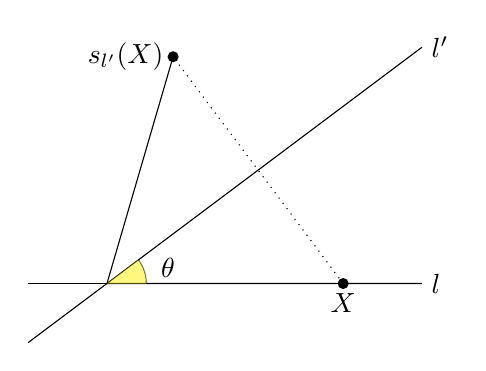
\begin{tikzpicture}
   % Draw axes
\coordinate (A) at (0,0);
\coordinate (B) at (4,0);
\coordinate (C) at (4,3);
\coordinate (D) at (-1,0);
\coordinate (E) at (-1,-3./4);
\coordinate (X) at (3,0);
\coordinate (XX) at (21/25, 72/25);


\fill (X) circle[radius=2pt] node[below] {$X$};
\fill (XX) circle[radius=2pt] node[left] {$s_{l^\prime}(X)$};
\draw[dotted] (X) -- (XX);
\draw[thin] (A) -- (XX);

\draw[thin] (B) node[right] {$l$} -- (A) -- (C) node[right] {$l^\prime$} ;
\draw[thin] (D) -- (A);
\draw[thin] (E) -- (A);
\path[clip] (C) -- (A) -- (B);
\fill[yellow, opacity=0.5, draw=black] (A) circle (5mm);
\node at ($(A)+(14:8mm)$) {$\theta$};
\end{tikzpicture}
\end{center}
\end{figure}
For å finne hvilken vinkel vi roterer med, er det nok å se hvor mye ett enkelt punkt blir rotert. Velg da dette punktet til å ligge på $l$. Da ser vi at origo (der vinkelen $\theta$ ligger) er toppen i en likebeint trekant med punktet $X$ og $s_{l^\prime}(X)$ som hjørner. Siden $l^\prime$ deler trekanten i to, må vinkelen være $2\theta$.

Til slutt: hva er sammensetningen av to speilinger om parallelle linjer? Kall linjene $l$ og $l^\prime$. De ligger da over hverandre i en avstand $\vec a$. Vi kan anta at den nederste linjen er $x$-aksen. Da blir også $s_l(\vec a)=-\vec a$. Legg merke til at om $l^\prime$ er "øverst", så er $s_{l^\prime}=t_{\vec a}s_l t_{-\vec a}$. Dermed er
$$
s s_{l^\prime} = s t_{\vec a} st_{-\vec a} = s^2 t_{s(\vec a)} t_{-\vec a} = t_{s(\vec a) - \vec a}=t_{-2\vec a}.
$$
Vi konkluderer med at en sammensetning av to speilinger er det samme som å translatere med en avstand det dobbelte av avstanden mellom linjene.
\end{losn}

\begin{oppg}
La $\ell$ være linjen gjennom origo med retningsvektor $(a,b)$ ($b > 0$). Skriv standardmatrisen til speilingen $s_{\ell}$. 
\end{oppg}
\begin{losn}
Vi tar først for oss tilfellet når $\ell$ er $x$-aksen. I det tilfellet er bare speilingen gitt ved 
$$ 
S = \begin{bmatrix}
1 & 0 \\ 0 & -1
\end{bmatrix}.
$$
Så strategien blir å først rotere linjen $\ell$ slik at den sammenfaller med $x$-aksen, og så bruke $S$, og så rotere tilbake til $\ell$.

Det er lett å se at matrisen 
$$ 
M_\theta = \frac{1}{\sqrt{a^2+b^2}} \begin{bmatrix}
a & -b \\ b & a
\end{bmatrix}.
$$
tar $x$-aksen på linjen $\ell$, er ortogonal og har determinant $1$. Dermed er $M_\theta$ en rotasjonsmatrise. Det er også greit å se at
$$ 
M_\theta^{-1} = M_{-\theta} = \frac{1}{\sqrt{a^2+b^2}} \begin{bmatrix}
a & b \\ -b & a
\end{bmatrix}.
$$

Vi regner dermed ut at speilingen gjennom linjen $\ell$ er gitt ved
$$
M_\theta S M_{-\theta} = \frac{1}{a^2+b^2} \begin{bmatrix}
a^2-b^2 & 2ab \\ 
2ab & b^2-a^2
\end{bmatrix}.
$$
PS: Om en slår opp på Wikipedia ser en at en formel for en slik speiling er gitt ved 
$$
\vec x \mapsto 2 \frac{\vec v \cdot \vec x}{\vec v \cdot \vec v} \vec v - \vec x,
$$
der $\vec v = (a,b)$. Men ved å se hva som skjer med enhetsvektorer er det lett å se at dette faktisk er samme formel.
\end{losn}

\begin{oppg}
Beskriv symmetrigruppene til:
\begin{enumerate}[a)]
\item En likebeint trekant.
\item En likesidet trekant.
\item En parabel.
\item Et parallellogram.
\item En rombe.
\item Et rektangel.
\item En ellipse.
\end{enumerate}
\end{oppg}

\begin{losn}
\begin{enumerate}[a)]
\item \textbf{En likebeint trekant}: Vi antar trekanten er likebeint, men ikke side likesidet. En slik trekant har bare to symmetrier: som alltid identiteten, og speiling gjennom en høyde.
\item \textbf{En likesidet trekant}: En likesidet trekant er den trekanten med flest symmetrier. Vi kan rotere $120^\circ$, og vi kan reflektere om hvert hjørne. Til sammen får vi seks symmetrier, den fulle trekantgruppen $D_3$.
\item \textbf{En parabel}: En parabel har heller ikke mange symmetrier. I det enkleste tilfellet er den gitt som $y=x^2$, og da ser vi at $x \mapsto -x$ er en symmetri, som svarer til speiling om $y$-aksen. Dette er da også den eneste symmetrien, og dette gjelder generelt (alle parabler kan ved hjelp av et koordinatskifte skrives om til noe på formen $y=x^2$). 
\item \textbf{Et parallellogram}: Vi antar parallellogrammet ikke er en rombe (det vil si, siden er av forskjellig lengde). Vi kan også anta at vi ikke har et rektangel. Men da er det lett å se at et parallellogram ikke har noen symmetrier.
\item \textbf{En rombe}: En rombe er et parallellogram hvor siden er like lange. I dette tilfellet er speiling lov: velg et hjørne, og speil gjennom linjen som går gjennom to hjørner. Dette gir til sammen fire symmetrier: identiteten, speiling i to nabohjørner hjørner, og sammensetningen av disse.
\item \textbf{Et rektangel}: Hvis rektangelet ikke er et kvadrat, er det bare speilinger vi kan gjøre. Så svaret blir 
akkurat det samme som med romben.
\item \textbf{En ellipse}: En ellipse har fire symmetrier, akkurat som rektangelet og romben. Grunnen til dette er at 
alle tre har to ``symmetriakser''.
\end{enumerate}

\end{losn}

\end{document}
